% 1977 年黑龙江初试卷第 7 题：⊙O 的两条切线 AB、AC，切点 B、C，∠BAC=120°（按源卷第 2 页布局）
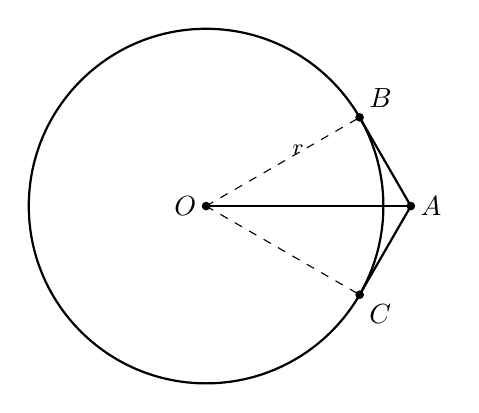
\begin{tikzpicture}[scale=1.3]
  \coordinate (O) at (0,0);
  \coordinate (A) at (2,0);
  \coordinate (B) at (1.5,0.866);
  \coordinate (C) at (1.5,-0.866);
  \draw[thick] (O) circle (1.732);
  \draw[thick] (A)--(B);
  \draw[thick] (A)--(C);
  \draw[thick] (O)--(A);
  \draw[dashed] (O)--(B);
  \draw[dashed] (O)--(C);
  \fill (O) circle (1.2pt) node[left] {$O$};
  \fill (A) circle (1.2pt) node[right] {$A$};
  \fill (B) circle (1.2pt) node[above right] {$B$};
  \fill (C) circle (1.2pt) node[below right] {$C$};
  \node at (0.9,0.55) {\footnotesize $r$};
\end{tikzpicture}
